
The field of exoplanets (``extra-solar planets'', or planets around other stars) has established itself as the hot new field in astrophysics. Since the discovery of the first exoplanets in the early 1990's \cite{pulsarplanet}, nearly 3000 exoplanets have been discovered \cite{exoplanetorg}, with potentially thousands more exoplanets remaining unconfirmed or thus far undiscovered in existent data.  This explosion in exoplanet discovery has been fueled by the funding and construction of many exoplanet detection surveys.  The majority of exoplanets have been found by the space-based {\it Kepler} telescope and its primary \cite{kepler} and ``K2'' surveys \cite{k2}.  Ground-based surveys, while not as sensitive to smaller planets as {\it Kepler} (due to atmospheric distortion of image quality and other problems associated with observing from the ground), are sufficiently sensitive to discover Jupiter-sized planets on short-period orbits.  Such planets are called ``hot Jupiters'' because they are the similar in size to Jupiter but are sufficiently close in to the stars they orbit (much closer than Mercury is to our sun) that the star heats them up to several thousands of degrees Celsius.

  Since ground-based surveys are much cheaper to run per area of sky monitored than spaced-based surveys, the majority of known hot Jupiters have been discovered by large-scale ground-based surveys.
Of the few hundred hot Jupiters that have been found to date, the plurality (${\sim}$100) have been found by Princeton's own Hungarian-made Automated Telescope (HAT) collaboration, headed by Prof. Gaspar Bakos of the Department of Astrophysical Sciences.  This collaboration runs two surveys. The longest-running of the two surveys is HATNet, a collection of five telescopes in Arizona and two telescopes in Hawaii \cite{hatnet}.  The other survey is HATSouth, which consists of three locations with eight telescopes each: Chile, Namibia, and Australia \cite{hatsouth}.  A third survey, HATPI, which will consist of 63 telescopes in Chile, is currently being constructed \cite{hatpi}.  The telescopes themselves are small as telescopes go: only about 10 cm across, they are more similar to camera lenses than the ``normal'' telescopes usually associated with astronomy.  Figure~\ref{hsscopes} shows a picture of four of the HAT-South telescopes.

\begin{figure}
\begin{centering}
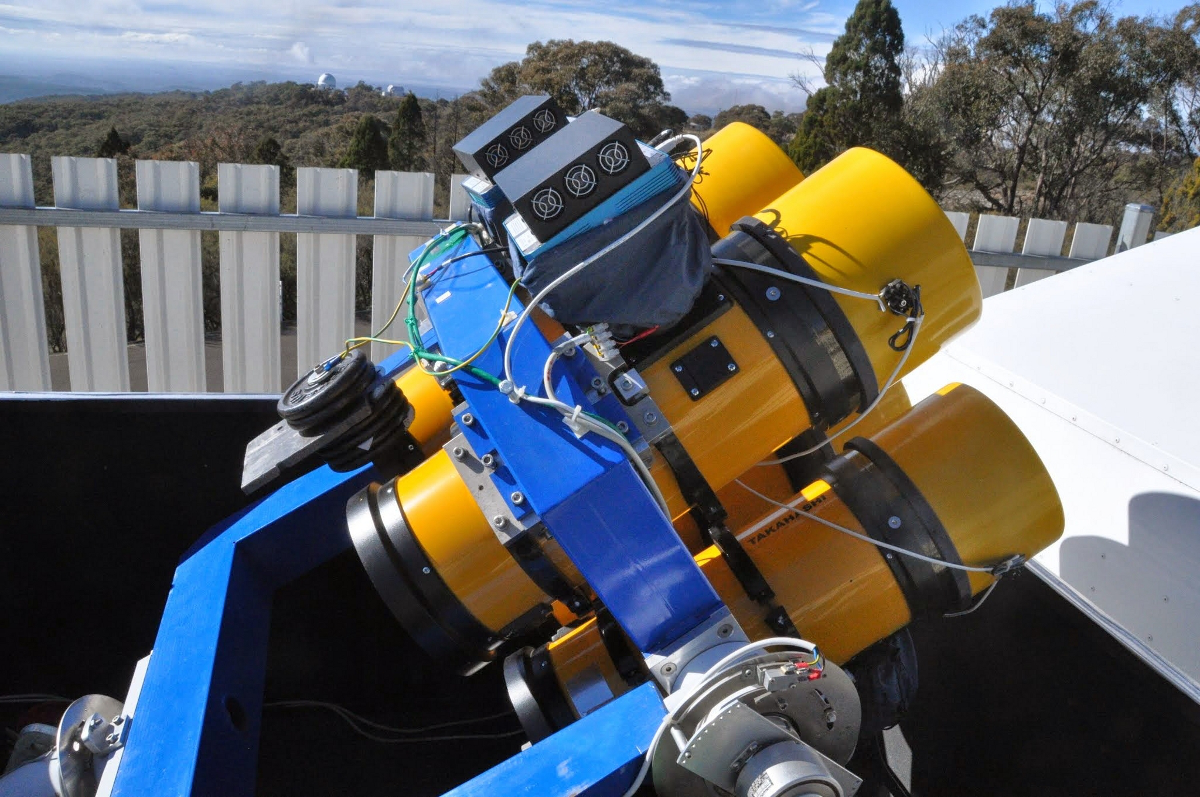
\includegraphics[width=3in]{hs-scopes.png}
\caption{\label{hsscopes} The four HATSouth telescopes at Siding Springs Observatory, Australia.  Photo credit Gaspar Bakos.  From \cite{hatsouthpicture}.}
\end{centering}
\end{figure}

The detection technique used by HAT*, {\it Kepler}, and many other exoplanet surveys is the ``transit'' technique.  Planets are far too faint compared to their host stars to be able to directly image around most stars.  Instead, in the transit technique, the brightness of stars is monitored as a function of time (usually by taking periodic long-exposure photographs of large areas of the sky).  When a planet crosses in front the star it orbits, the amount of light detected from that star is decreased.  This is demonstrated cartoon-style in Figure~\ref{transit}.  Transits are found in data using matched filtering (with either a box- or trapezoid-shaped filter, matching the signal from a transiting exoplanet), folding the data on a variety of periods and phases.  When a star is found to have periodic dips in brightness, it is labeled as a potentially planet-hosting star.  However, transiting planets are not the only source of periodic signals like that seen in Figure~\ref{transit}.  Starspots rotating in and out of view also provide periodic dips in brightness and binary stars that eclipse each other in a grazing way (so the amount of light that goes missing during an eclipse is about the same as a planet) are two examples of astrophysical false positive signals. Various cuts are made to help ensure that a prospective planet is neither any of these false positives nor a spurious signal.  The various parameters of the fit to the transit signal (depth, time of ingress, length of transit) are often good indicators to separate between planet and not.  These cuts are automated.  However, after the cuts, there are still false positives that are not apparent to the pipeline but are obvious to a trained human eye.  Thus, the final step in the HAT pipeline is a manual, by-eye examination of the signal.  Planet candidates that pass this step then are sent for follow up (and hopefully confirmation!) at bigger telescopes.

\begin{figure}
\begin{centering}
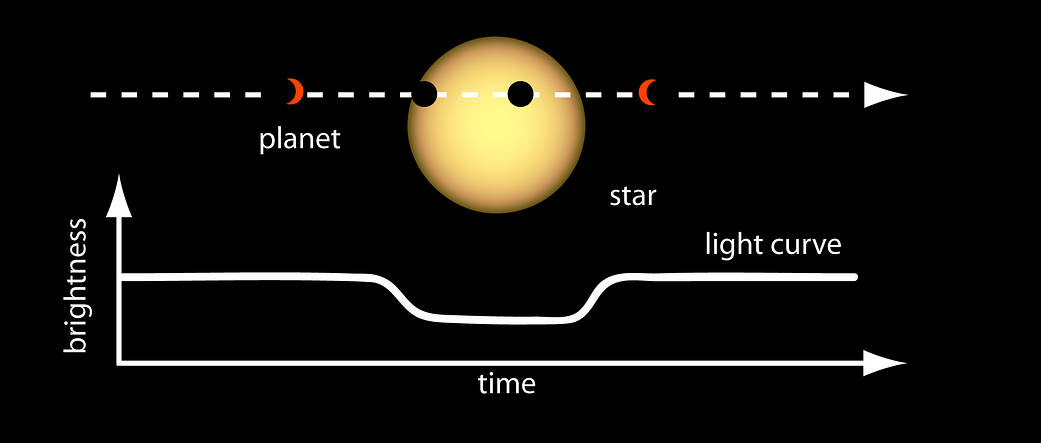
\includegraphics[height=1.9in]{transit.png}
\caption{\label{transit} An example ``light curve'' (brightness as a function of time) from a star that hosts a transiting exoplanet.  As the planet crosses in front of the star, the measured brightness from the star is less than the out-of-transit value.  Partial eclipses as the planet is transitioning from being out-of-transit to fully in transit put a slope in the light curve between in-transit and out-of-transit magnitudes.  Public domain image from \cite{transit_pic}.}
\end{centering}
\end{figure}

Other than this manual step, the vetting of possible planet candidates is completely automatic.  This single manual step is quite labor intensive, and prevents a fully automatic characterization of planet detection efficiency (what fraction of real planets get correctly identified), which is necessary for the calculation of statistics related to the occurrence rate of these planets.  Thus, it would be very nice to have an automated approximation to the by-eye work that has occurred.  This is the purpose of this project.